\documentclass[a4paper, 12pt]{article}
\usepackage[utf8]{inputenc}
\usepackage[T1,T2A]{fontenc}
\usepackage[a4paper, top=2cm, bottom=2cm, left=1cm, right=1cm, marginparwidth=1.75cm]{geometry}
\usepackage{graphicx}
\usepackage{amsmath}
\usepackage{indentfirst}
\usepackage[english, russian]{babel}
\usepackage[section,above,below]{placeins}
\usepackage[noend]{algorithmic}
\usepackage{amssymb}
\usepackage{amsfonts}
\usepackage{pdfpages}

\newcommand{\df}[2]{\frac{\partial #1}{\partial #2}}

\begin{document}
\section{Лабораторная 1}
{\bf Дана задача}:
\begin{equation}
    \dfrac{\partial K(t)}{\partial t}=L(t)+3K(t), K(0)=2,0\le L < \infty, t \in [0,2]
\end{equation}    
\begin{equation}
    I(K,L)=\int_0^2 K(t)+L^2(t) dt - 2 K(2) \rightarrow \min.
\end{equation}

{\bf Решение}:

Оптимальный процесс является решением вспомогательной задачи
\begin{equation}
    H(K,L,p)=-(K+L^2)+p(L+3K)\rightarrow \max_L,
\end{equation}
то есть 
\begin{equation}
   \df{H}{L}=-2L+p=0 \Rightarrow L=\frac{p}{2}.
\end{equation}

Сопряженная задача имеет вид:
\begin{equation}
    \dot p = -\df{H}{K}=1-3p,
\end{equation}
\begin{equation}
    p(2)=-\df{(-2K(2))}{K(2)}=2.
\end{equation}
{\bf Расчётная часть} представлена на рис. \ref{11beg}-\ref{11end}.
\begin{figure}[h]
    \noindent\centering{
    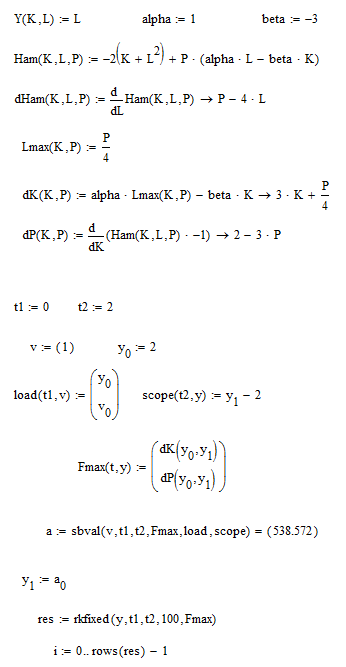
\includegraphics{11beg.png}
    }
    \caption{Расчёты}
    \label{11beg}
\end{figure}
\begin{figure}[h]
    \noindent\centering{
    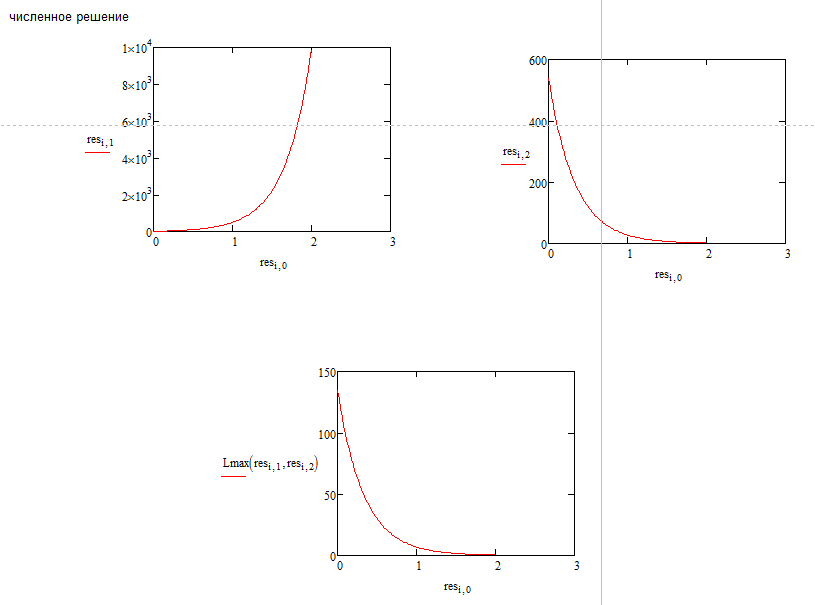
\includegraphics[width=0.99\linewidth]{11end.png}
    }
    \caption{Графики численного решения}
    \label{11end}
\end{figure} 

Дифференциальное уравнение имеет решение $p=C_1 \dfrac{e^{-3t}}{3} +\dfrac{1}{3}$, причем $p(2)=2$, поэтому $C_1=5 e^{6}$, тогда
\begin{equation}
    p(t)=\dfrac{1}{3}\left(5e^{6} e^{-3t}+1 \right) ,
\end{equation}
\begin{equation}
    L(t)=\dfrac{1}{6}\left(5e^{6} e^{-3t}+1 \right)>0,
\end{equation}
\begin{equation}
    \df{K}{t}=3K+\dfrac{5}{6} e^{-3t+6}+\dfrac{1}{6} \Rightarrow K=\left(C_1- \dfrac{c e^{-3t}}{3}- \dfrac{k e^{-6t}}{6}\right) e^{3t},c=\dfrac{1}{6},k=\dfrac{5 e^{6}}{6}.
\end{equation}

Из условия $K(0)=2$ находим $C_1=2\dfrac{1}{18}+\dfrac{5 e^{6}}{36}$, откуда 
\begin{equation}
    K(t)=K=\left(2\dfrac{1}{18}+\dfrac{5 e^{6}}{36}- \dfrac{e^{-3t}}{18}-\dfrac{5 e^{6} e^{-6t}}{36}\right) e^{3t}.
\end{equation}
{\bf Расчётная часть} представлена на рис. \ref{12beg}-\ref{12end}.
\begin{figure}[h]
    \noindent\centering{
    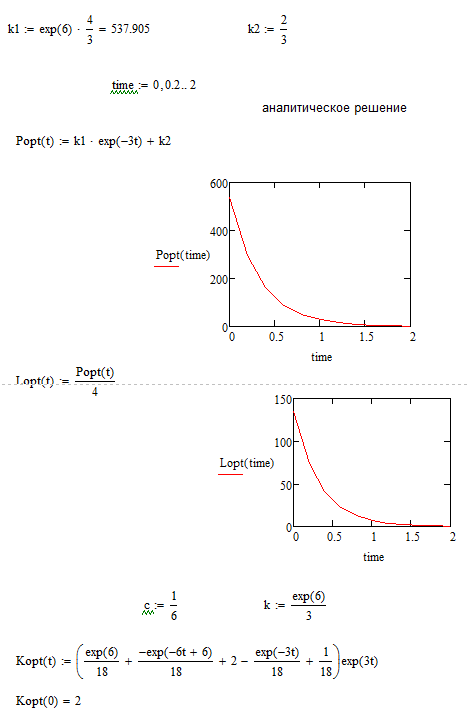
\includegraphics{12beg.png}
    }
    \caption{Графики аналитического решения}
    \label{12beg}
\end{figure}
\begin{figure}[h]
    \noindent\centering{
    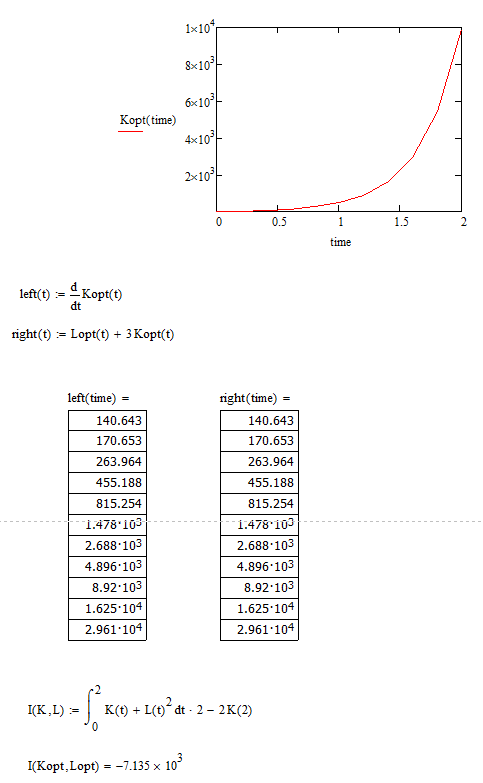
\includegraphics[width=0.6\linewidth]{12end.png}
    }
    \caption{Графики аналитического решения}
    \label{12end}
\end{figure} 

\section{Лабораторная 2}

{\bfЗадача}:
\begin{equation}
    \begin{cases}
        \dot x_1 =x_2, & x_1(0)=1,\\
        \dot x_2=x_1+u,& x_2(0)=1, t \in [0,10]
    \end{cases}
\end{equation}
\begin{equation}
    I=\int_0^{10} u^2 - x_1 dt \rightarrow \min.
\end{equation}

{\bf Решение}:

Задача для функции Гамильтона
\begin{equation}
    H=x_1-u^2 +p_1 x_2 +p_2 (x_1 +u) \rightarrow \max_u
\end{equation}
имеет решение 
\begin{equation}
    \df{H}{u}=-2u+p_2=0 \Rightarrow u=\dfrac{p_2}{2}.
\end{equation}
Для сопряжённых переменных система дифференциальных уравнений
\begin{equation}
    \begin{cases}
       \dot p_1 = - \df{H}{x_1}=-1-p_2, & p_1(10)=0,\\
       \dot p_2 = - \df{H}{x_2}=-p_1, & p_2(10)=0
    \end{cases}
\end{equation}
имеет решение в виде
\begin{equation}
    \begin{cases}
        p_1= C_1 e^t - C_2 e^{-t},\\
        p_2 = -C_1 e^t - C_2 e^{-t} -1,
    \end{cases}
\end{equation}
где $C_1 = -\dfrac{e^{-10}}{2},C_2 = -\dfrac{e^{10}}{2}$. Тогда система для ${\bf x}$ имеет вид
\begin{equation}
    \begin{cases}
        \dot x_1 =x_2, & x_1(0)=1,\\
        \dot x_2=x_1+\dfrac{e^{-10}}{4}e^t + \dfrac{e^{10}}{4}e^{-t}-\dfrac{1}{2},& x_2(0)=1.
    \end{cases}
\end{equation}
{\bf Расчётная часть} представлена на рис. \ref{21beg}-\ref{21end}.
\begin{figure}[h]
    \noindent\centering{
    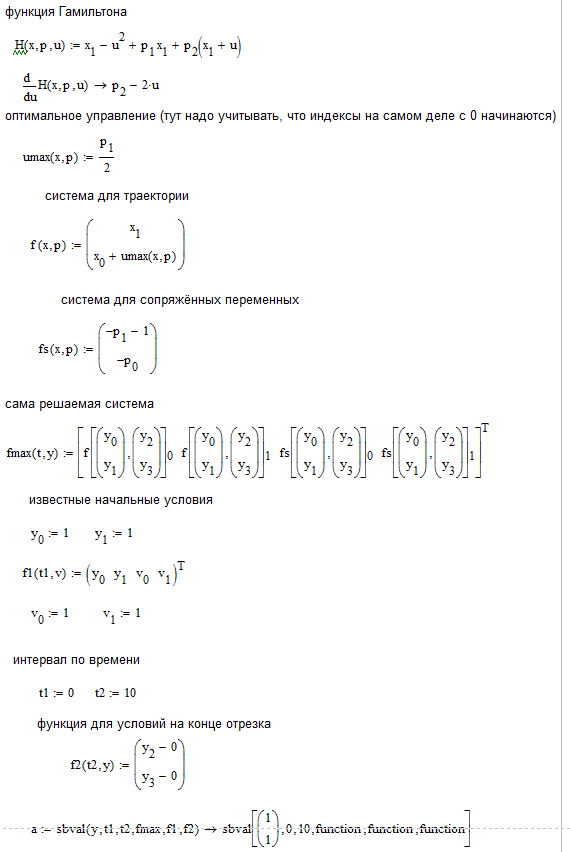
\includegraphics{21beg.png}
    }
    \caption{Расчёты}
    \label{21beg}
\end{figure}
\begin{figure}[h]
    \noindent\centering{
    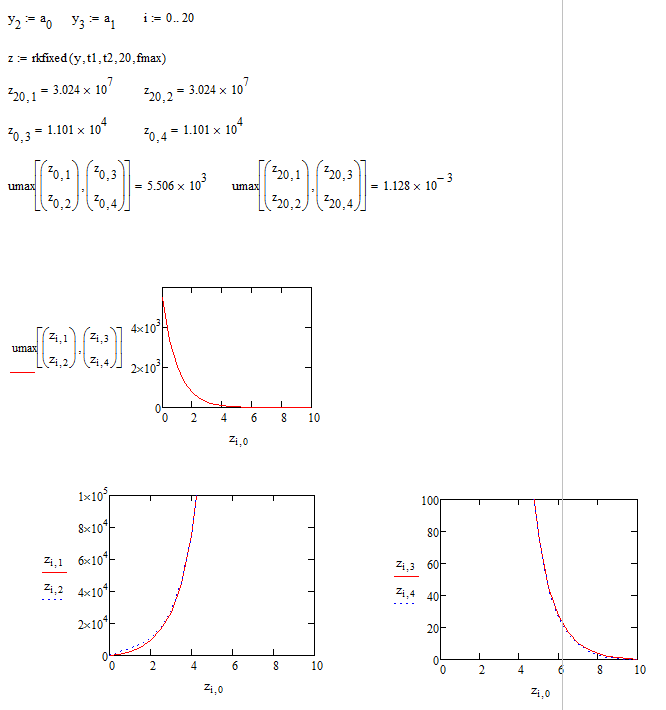
\includegraphics[width=0.99\linewidth]{21end.png}
    }
    \caption{Графики численного решения}
    \label{21end}
\end{figure} 

Введём константы $a=\dfrac{e^{-10}}{4},b=\dfrac{e^{10}}{4},c=-\dfrac{1}{2}$, тогда общее решение системы имеет вид
\begin{equation}
    \begin{cases}
        x_1 =\dfrac{1}{4}\left(a e^t (2t-1) - b e^{-t} (2t+1)-4c  \right) +\dfrac{1}{2} C_1 (e^t + e^{-t}) + \dfrac{1}{2} C_2 (e^t - e^{-t}),\\
        x_2=\dfrac{1}{4} e^{-t} \left(a e^{2t} (2t+1) +b (2t-1) \right) +\dfrac{1}{2} C_1 (e^t-e^{-t})+\dfrac{1}{2} C_2 (e^t + e^{-t}).
    \end{cases}
\end{equation}

Из граничных условий находим: $C_1=1+\dfrac{1}{4}(a+b+4c),C_2 = 1+\dfrac{1}{4}(b-a)$.
{\bf Расчётная часть} представлена на рис. \ref{22}.
\begin{figure}[h]
    \noindent\centering{
    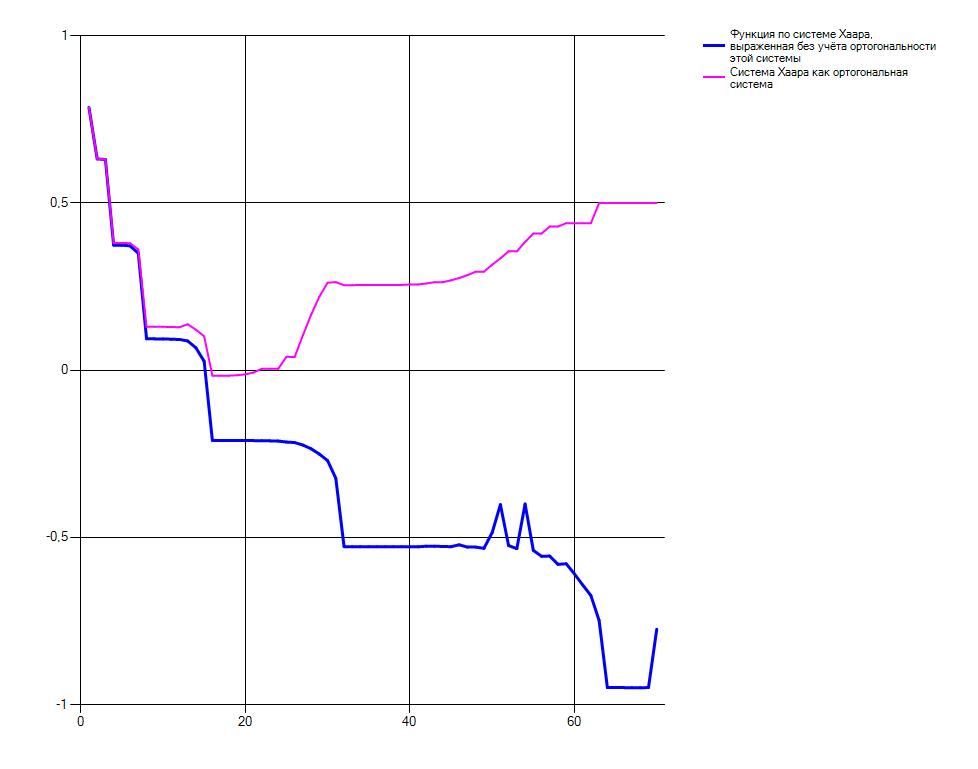
\includegraphics[width=0.99\linewidth]{22.png}
    }
    \caption{Графики аналитического решения}
    \label{22}
\end{figure} 

\section{Лабораторная 3}
{\bf Задача}:
\begin{equation}
    \dot x = x+u , 0\leq u \leq 3, x(0)=1, t \in [0,4],
\end{equation}
\begin{equation}
    I=\int_0^4 3 u dt - x(4) \rightarrow \min.
\end{equation}
{\bf Решение}:

Из задачи для функции Гамильтона 
\begin{equation}
    H=-3u+p(x+u)=u(p-3)+px \rightarrow \max
\end{equation}
следует
\begin{equation}
    u=
    \begin{cases}
        3, & p-3 >0,\\
        0, & p-3<0
    \end{cases} 
    \Leftrightarrow
    \begin{cases}
        3, & p >3,\\
        0, & p<3
    \end{cases} 
\end{equation}

Для $p$ имеем задачу
\begin{equation}
    \dot p = - \df{H}{x}=-p,p(4)=-\df{(-x(4))}{x(4)}=1,
\end{equation}
откуда 
\begin{equation}
    p=C_1 e^{-t} \Rightarrow p(4) = C_1 e^{-4} = 1 \Rightarrow C_1=e^4 \Rightarrow p= e^4 e^{-t}.
\end{equation}
{\bf Расчётная часть} представлена на рис. \ref{31}.
\begin{figure}[h]
    \noindent\centering{
    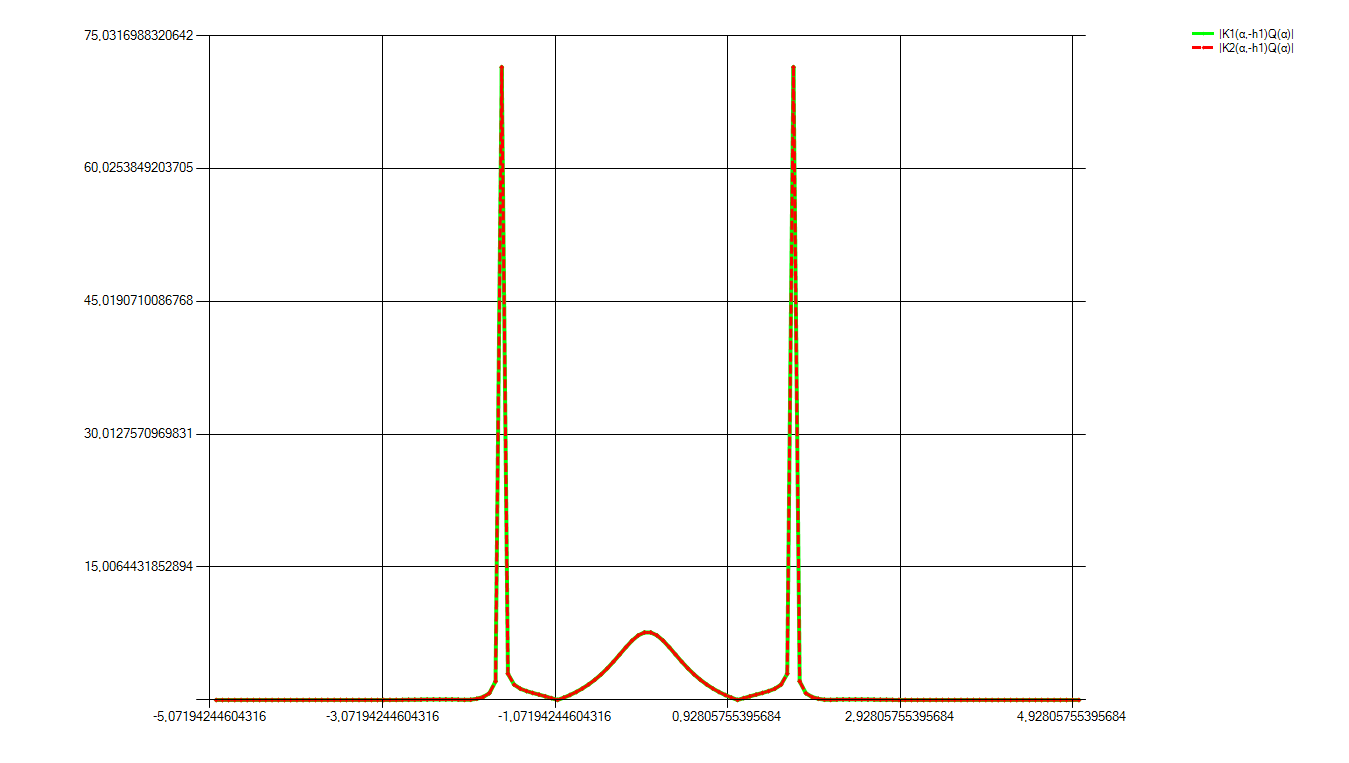
\includegraphics[width=0.7\linewidth]{31.png}
    }
    \caption{Графики численного решения}
    \label{31}
\end{figure}

Тогда $p=3$ при $t=4-\ln 3$. Поскольку функция $p$ убывающая, функция $u$ принимает вид
\begin{equation}
    u=
    \begin{cases}
        3, & t \in [0,4-\ln 3],\\
        0, & t \in [4-\ln 3,4]
    \end{cases} 
\end{equation}
Из уравнения $\dot x = x +u$ следует $x=C_1 e^t -u$. Тогда на отрезке $t \in [0,4-\ln 3]$ решается задача
\begin{equation}
    x=C_1 e^t -3,x(0)=1 \Rightarrow C_1 -3 =1 \Rightarrow C_1=4 \Rightarrow x=4 e^t -3, x(4-\ln 3)=\dfrac{4}{3} e^4 -3.
\end{equation}
Аналогично для отрезка $t \in [4-\ln 3,4]$:
\begin{equation}
    x=C_1 e^t,x(4-\ln 3)=\dfrac{4}{3} e^4 -3 \Rightarrow C_1 = e^{\ln 3 - 4} \left(\dfrac{4}{3} e^4 -3  \right)=4- 9 e^{-4} \Rightarrow x=(4-9e^{-4})e^t.
\end{equation}
В итоге для траектории:
\begin{equation}
    \begin{cases}
        x=4 e^t -3, & t \in [0,4-\ln 3],\\
        x=(4-9e^{-4})e^t & t \in [4-\ln 3,4].
    \end{cases}
\end{equation}

{\bf Расчётная часть} представлена на рис. \ref{32}.
\begin{figure}[h]
    \noindent\centering{
    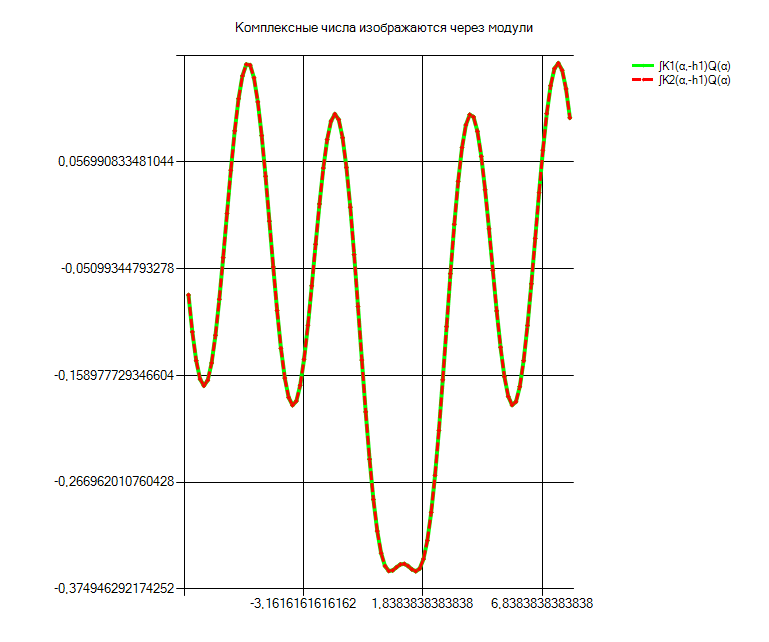
\includegraphics[width=0.9\linewidth]{32.png}
    }
    \caption{Графики аналитического решения}
    \label{32}
\end{figure}

\section{Лабораторная 4}

{\bfЗадача}:
\begin{equation}
    \begin{cases}
        \dot x_1 =-x_2, & x_1(0)=1,\\
        \dot x_2=-x_1+u,& x_2(0)=2, t \in [0,1], 0\leq u \leq 2
    \end{cases}
\end{equation}
\begin{equation}
    I=\int_0^{1} x_2 + u dt +x_2(1) \rightarrow \min.
\end{equation}

{\bf Решение}:

Из задачи для функции Гамильтона:
\begin{equation}
    H=-u-x_2-p_1 x_2 + p_2 (u-x_1)=(p_1-1) u - p_1 x_2 -p_2 x_1 -x_2 \rightarrow \max_u
\end{equation}
следует
\begin{equation}
    u=
    \begin{cases}
        2,&p_2>1\\
        0,&p_2<1
    \end{cases}.
\end{equation}

Задача для сопряженных переменных
\begin{equation}
    \begin{cases}
        \dot p_1 = -\df{H}{x_1}=p_2, &p_1(1)=0\\
        \dot p_2=- \df{H}{x_2}=p_1+1, &p_2(1)=-\df{(x_2(1))}{x_2(1)}=-1
    \end{cases}
\end{equation}
имеет решение
\begin{equation}
    \begin{cases}
        p_1=\dfrac{1}{2}C_1 (e^t+e^{-t})+\dfrac{1}{2} C_2 (e^t-e^{-t})-1,\\
        p_2=\dfrac{1}{2}C_1 (e^t-e^{-t})+\dfrac{1}{2} C_2 (e^t+e^{-t})
    \end{cases},
\end{equation}
где $C_1=e,C_2=-e$. В сокращённом виде:
\begin{equation}
    \begin{cases}
        p_1=e \cdot e^{-t}-1,\\
        p_2=-e \cdot e^{-t}
    \end{cases}.
\end{equation}
{\bf Расчётная часть} представлена на рис. \ref{41beg}-\ref{41end}.
\begin{figure}[h]
    \noindent\centering{
    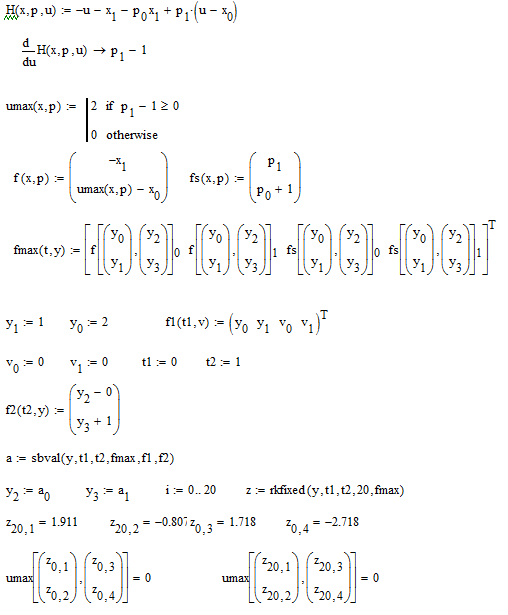
\includegraphics{41beg.png}
    }
    \caption{Расчёты}
    \label{41beg}
\end{figure}
\begin{figure}[h]
    \noindent\centering{
    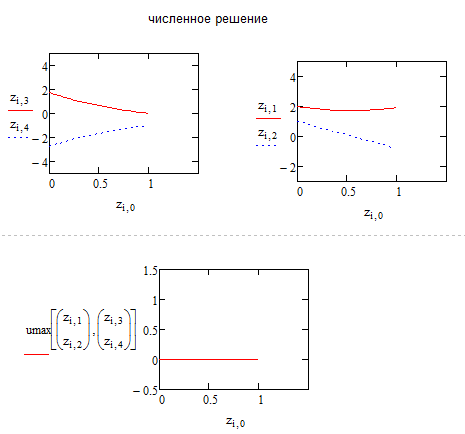
\includegraphics[width=0.8\linewidth]{41end.png}
    }
    \caption{Графики численного решения}
    \label{41end}
\end{figure} 

Очевидно, что $p_2<0$ всегда, откуда $u=0$. В этом случае система дифференциальных уравнений для ${\bf x}$ имеет решение
\begin{equation}
    \begin{cases}
        x_1=C_1 e^t + C_2 e^{-t},\\
        x_2=-C_1 e^t + C_2 e^{-t}
    \end{cases},
\end{equation}
где $C_1=-0.5$, $C_2=1.5$.

{\bf Расчётная часть} представлена на рис. \ref{42}.
\begin{figure}[h]
    \noindent\centering{
    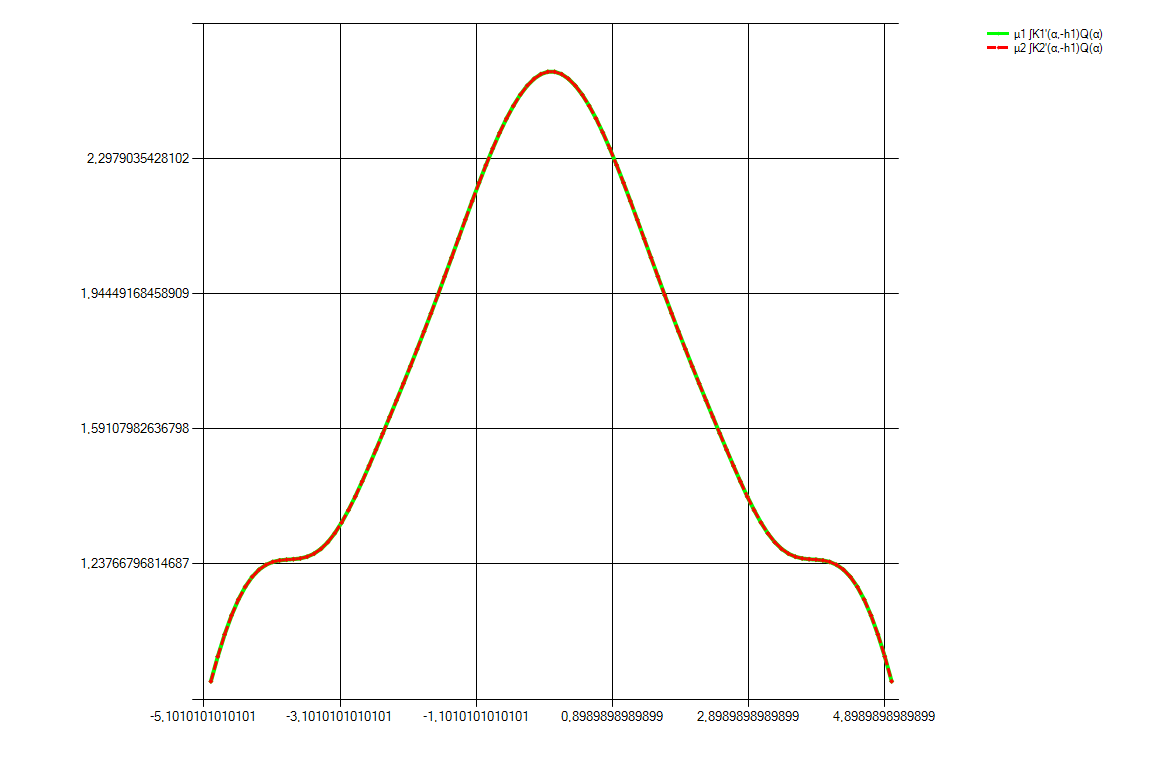
\includegraphics[width=0.8\linewidth]{42.png}
    }
    \caption{Графики аналитического решения}
    \label{42}
\end{figure} 

\section{Лабораторная 5}
{\bf Задача}:
\begin{equation}
    \dot x = u , x(0)=-1, t \in [0,3],
\end{equation}
\begin{equation}
    I=\int_0^3 u^2+x dt - x(3) \rightarrow \min.
\end{equation}

{\bf Решение}:
Из задачи
\begin{equation}
    R= \df{\varphi}{t}+\df{\varphi}{x} u - u^2-x \rightarrow \max_u
\end{equation}
находим, что
\begin{equation}
    \df{R}{u}=\df{\varphi}{x} - 2u \Rightarrow u= \dfrac{1}{2} \df{\varphi}{x}.
\end{equation}

Поскольку терминальная функция $F(x)=-x$ является многочленом первого порядка, то функцию $\varphi(t,x)$ будем искать в виде $\varphi(t,x)=p(t)\cdot x$, откуда
\begin{equation}
    \df{\varphi}{t}= \df{p}{t} \cdot x, \df{\varphi}{x}=p. 
\end{equation}

Из уравнения для $p$
\begin{equation}
    P(x,t)=R|_{u=\frac{1}{2} \df{\varphi}{x}}=\df{\varphi}{t}+\dfrac{1}{2} \left(\df{\varphi}{x} \right)^2-\dfrac{1}{4} \left(\df{\varphi}{x} \right)^2-x=\left(\df{p}{t}-1 \right) +\dfrac{1}{4}p^2=c(t)
\end{equation}
получается уравнение
\begin{equation}
    \dot p=1
\end{equation}
при граничном условии
\begin{equation}
    \Phi (X) = \varphi (T,X)+F(x)=p(3) x-x=0 \Rightarrow p(3)=1.
\end{equation}

Для $x$ получаем уравнение $\dot x = \dfrac{1}{2} p$ при граничном условии $x(0)=-1$. Система этих уравнений имеет решение
\begin{equation}
    \begin{cases}
        p=t-2,\\
        x=\dfrac{t^2}{2}-t-1.
    \end{cases}
\end{equation}

{\bf Расчётная часть} представлена на рис. \ref{51beg}-\ref{51end}.
\begin{figure}[h]
    \noindent\centering{
    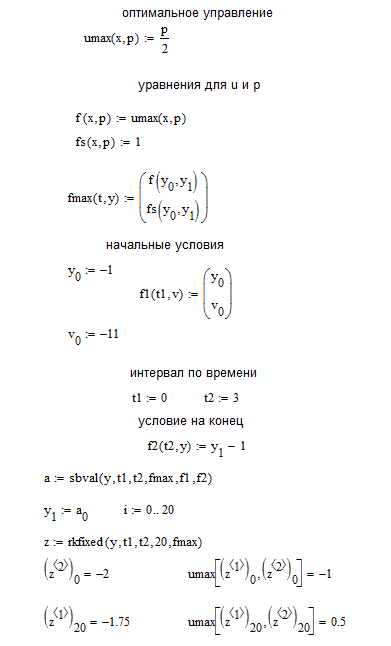
\includegraphics{51beg.png}
    }
    \caption{Расчёты}
    \label{51beg}
\end{figure}
\begin{figure}[h]
    \noindent\centering{
    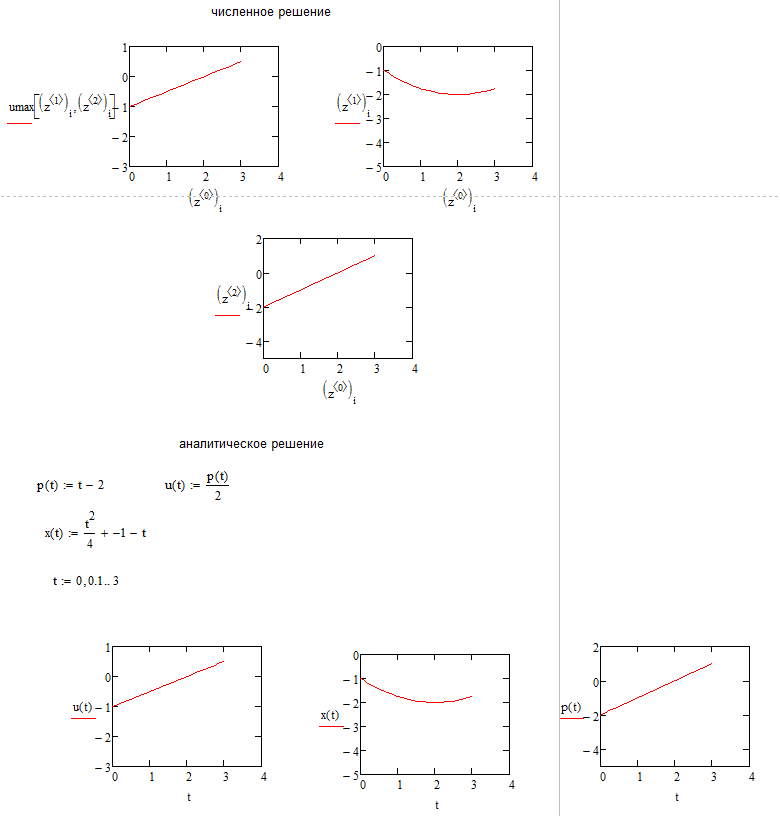
\includegraphics[width=0.9\linewidth]{51end.png}
    }
    \caption{Графики решения}
    \label{51end}
\end{figure} 

\section{Лабораторная 6}
{\bf Задача}:
\begin{equation}
    \dot x = -x+u , -1\leq u \leq 0, x(0)=1, t \in [0,2],
\end{equation}
\begin{equation}
    I=\int_0^2 x-u dt - 3x(2) \rightarrow \min.
\end{equation}
{\bf Решение}:

Из уравнения
\begin{equation}
    R=u-x +\df{\varphi}{x}(-x+u)+\df{\varphi}{t}
\end{equation}
получаем
\begin{equation}
    \df{R}{u}=1+\df{\varphi}{x} \Rightarrow u=
    \begin{cases}
        0,&\df{\varphi}{x} >-1,\\
        -1,&\df{\varphi}{x}<-1
    \end{cases}.
\end{equation}

Аналогично заданию 5 получаем, что $\varphi(t,x)=p(t)\cdot x$, откуда для $p>1$
\begin{equation}
    P(x,t)=-x(1+p)+\dot p x=c(t) \Rightarrow \dot p=p+1
\end{equation}
и
\begin{equation}
    p(2)x-3x=0 \Rightarrow p(2)=3.
\end{equation}

К этому уравнению добавляется
\begin{equation}
    \dot x=-x, x(0)=2.
\end{equation}

Решение полученной системы имеет вид
\begin{equation}
    \begin{cases}
        x=2 e^{-t},\\
        p=4 e^{t-2}-1 \geq -1
    \end{cases}
\end{equation}

{\bf Расчётная часть} представлена на рис. \ref{61beg}-\ref{61end}.
\begin{figure}[h]
    \noindent\centering{
    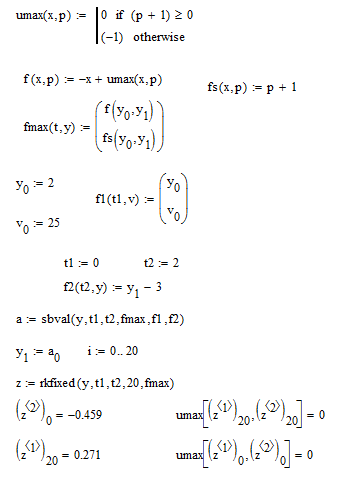
\includegraphics{61beg.png}
    }
    \caption{Расчёты}
    \label{61beg}
\end{figure}
\begin{figure}[h]
    \noindent\centering{
    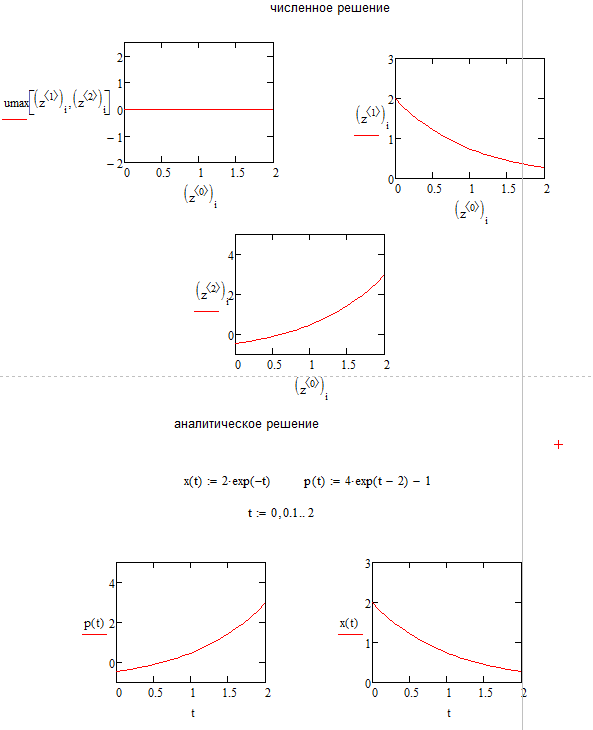
\includegraphics[width=0.9\linewidth]{61end.png}
    }
    \caption{Графики решения}
    \label{61end}
\end{figure} 

Для $p>1$ получим такое же уравнение для $p$ с таким же решением $p \geq -1$
\begin{equation}
    P(x,t)=-1-x +p(-x-1)+\dot p x=-1 -x(1+p)-p+\dot p x=c(t) \Rightarrow \dot p=p+1,
\end{equation}
откуда следует, что $x$ искать не имеет смысла и $u=0$ всегда.

\end{document}